\lab{Data Visualization}{Data Visualization} 
\objective{Use visualizations to explore and communicate insights in data.}
\label{lab:DataVis}

%\noindent\emph{At their best, graphics are instruments for reasoning about quantitative information.} \small{---Edward Tufte}
% from the introduction of his book 'The Visual Display of Quantitative Information'

\section*{Exploring Data with Visualizations} % ===============================

Using visualizations to understand data can reveal insights that may not be noticed otherwise.
The following problem is a famous example of this phenomenon.

\begin{problem} % Problem: Anscombe data set.
\label{prob:anscombe}
Consider the following data sets:
\begin{table}[H]
\begin{tabular}{l l  |  l l  |  l l  |  l l }
I & & II & & III & & IV\\
x & y & x & y & x & y & x & y \\
\hline
10.0 & 8.04 & 10.0 & 9.14 & 10.0 & 7.46 & 8.0 & 6.58 \\
8.0 & 6.95 & 8.0 & 8.14 & 8.0 & 6.77 & 8.0 & 5.76 \\
13.0 & 7.58 & 13.0 & 8.74 & 13.0 & 12.74 & 8.0 & 7.71 \\
9.0 & 8.81 & 9.0 & 8.77 & 9.0 & 7.11 & 8.0 & 8.84 \\
11.0 & 8.33 & 11.0 & 9.26 & 11.0 & 7.81 & 8.0 & 8.47 \\
14.0 & 9.96 & 14.0 & 8.10 & 14.0 & 8.84 & 8.0 & 7.04 \\
6.0 & 7.24 & 6.0 & 6.13 & 6.0 & 6.08 & 8.0 & 5.25 \\
4.0 & 4.26 & 4.0 & 3.10 & 4.0 & 5.39 & 19.0 & 12.50 \\
12.0 & 10.84 & 12.0 & 9.13 & 12.0 & 8.15 & 8.0 & 5.56 \\
7.0 & 4.82 & 7.0 & 7.26 & 7.0 & 6.42 & 8.0 & 7.91 \\
5.0 & 5.68 & 5.0 & 4.74 & 5.0 & 5.73 & 8.0 & 6.89 \\
\end{tabular}
\caption{These four sets of data are known as Anscombe's quartet.}
\label{table:anscombe}
\end{table}

The data sets I-IV in Table \ref{table:anscombe} are known as Anscombe's quartet. 
Each data set has identical statistical properties. 
In each case,
\begin{itemize}
\item The mean of $x$ is 9 and the mean of $y$ is $7.5$.
\item The variance of $x$ is 11 and the variance of $y$ is 4.127.
\item The correlation between $x$ and $y$ is .816.
\item The linear regression line is $y=3+5x$.
\end{itemize}
Plot each data set.
What do you notice? % TODO: ask a more specific question?
\end{problem}

\subsection*{The Iterative Process of Exploratory Visualization} % ------------

As Problem \ref{prob:anscombe} demonstrates, a picture quickly reveals properties of the data that are difficult to see in a list of numbers.
Understanding a data set through visualization is an iterative process.
Start with an initial visualization---usually a broad overview---and examine the data.
Adjust the visualization or create other visualizations based on what you observe.
Ask questions as you look for insights; this will help you find the right visualization.

Some good questions to ask include:
\begin{enumerate}
\item Does the data make sense?
\item Would a different visualization give more information?
\item Would visualizing a subset of the data provide more information?
\item Would transforming the data reveal a hidden pattern?
\end{enumerate}

\begin{figure}[H] % Different visuaizations for earthquake data. 
\centering
\begin{subfigure}{.45\textwidth}
\centering
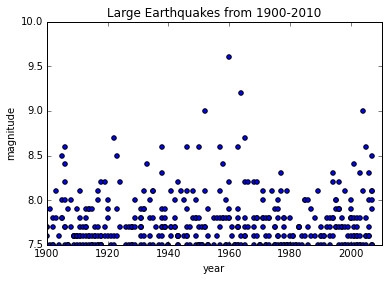
\includegraphics[width=\textwidth]{large_quake.png}
\end{subfigure}
\centering
\begin{subfigure}{.45\textwidth}
\centering
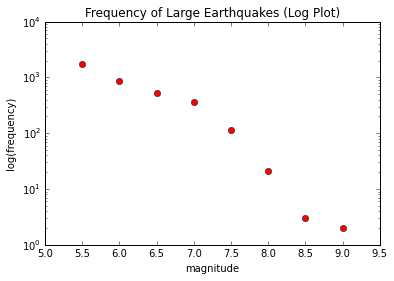
\includegraphics[width=\textwidth]{freq_earthquake_log.png}
\end{subfigure}
\caption{The left plot shows earthquakes of magnitudes 7.5 or higher over time. The right plot shows the frequencies of
different magnitudes. Note the scale of the y-axis is logarithmic.}
\label{fig:logexample}
\end{figure}

This last question is particularly important.
Consider Figure \ref{fig:logexample} which shows data about large earthquakes from the United States Geological Survey.
It appears to be somewhat random however, when transformed, the frequency of the magnitudes on a logarithmic scale show a fairly strong linear relationship
between the variables.
Transformations and data exploration will be discussed more in Volume 3.

\newpage

\subsection*{Types of Visualizations} % ---------------------------------------

\subsubsection*{Bar Charts} % -------------------------------------------------

\begin{figure}[H] % Bar chart styles
\centering
\begin{subfigure}{.45\textwidth}
  \centering
  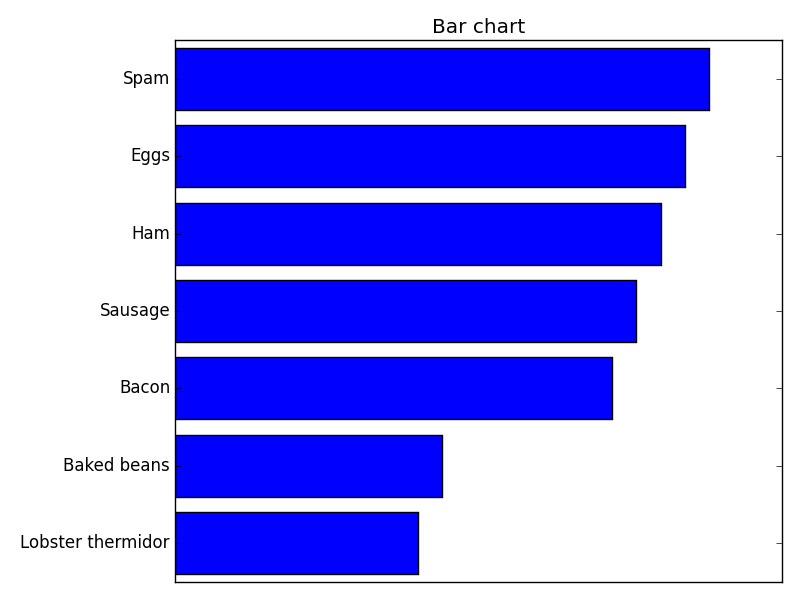
\includegraphics[width=\textwidth]{bar_chart_horizontal_sorted.png}
\end{subfigure}
\begin{subfigure}{.45\textwidth}
  \centering
  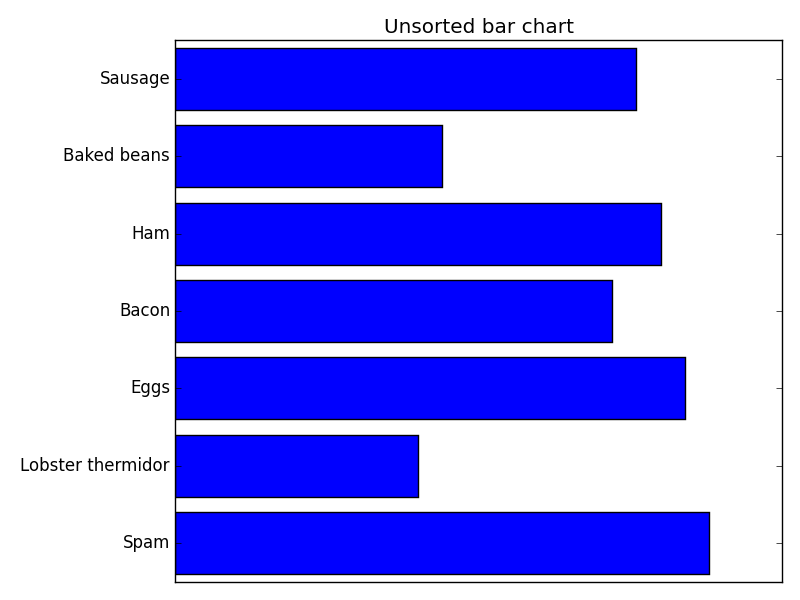
\includegraphics[width=\textwidth]{bar_chart_unsorted.png}
\end{subfigure}
\begin{subfigure}{.45\textwidth}
  \centering
  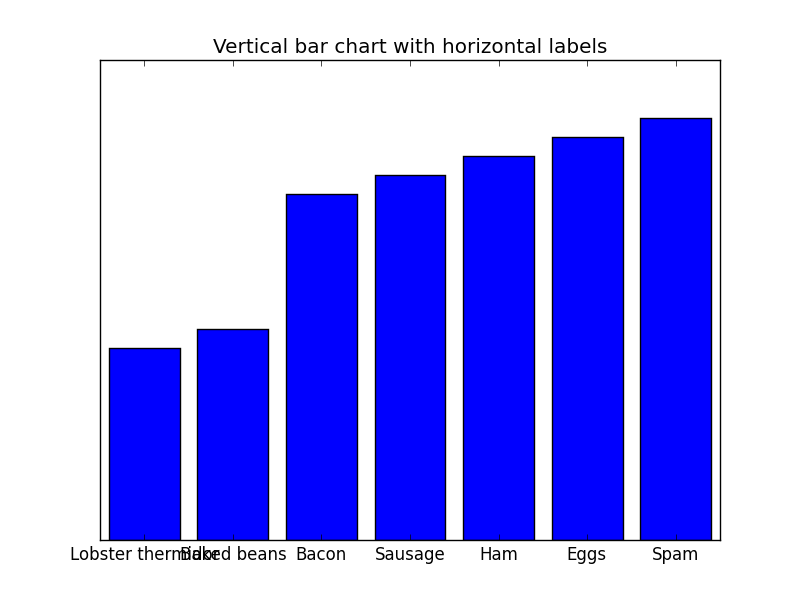
\includegraphics[width=\textwidth]{bar_chart_vertical_bars_horizontal_labels.png}
\end{subfigure}
\begin{subfigure}{.45\textwidth}
  \centering
  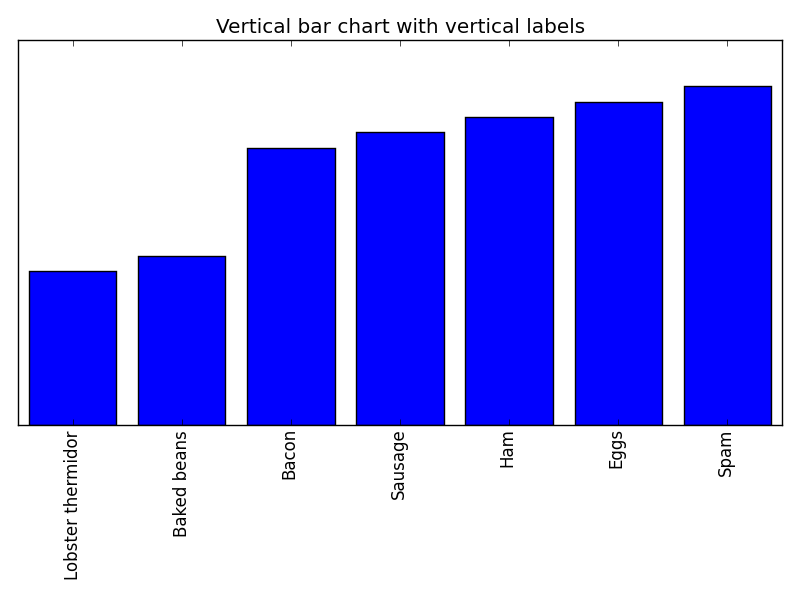
\includegraphics[width=\textwidth]{bar_chart_vertical_bars_vertical_labels.png}
\end{subfigure}

\caption{Bar Charts.
The example in the upper left is easier to use for comparison than the upper right, and easier to read than the bottom two charts.
The labels overlap in the bottom left and the labels are vertical in the bottom right, making them hard to read.}
\label{fig:barchart}
\end{figure}

Bar charts are best for small sets of discrete, one-dimensional, categorical data.
Usually, a horizontal bar chart is preferred over a vertical bar chart because it's harder to read vertical labels than horizontal labels.
Also, horizontal labels on a vertical bar chart may not fit on the graph well (see Figure \ref{fig:barchart}).

The data in a bar chart should be sorted in a logical way.
If the chart is being used to compare the values of different data points, it is best to sort by size; if the chart is being used to look up specific values, the labels should be sorted in a way that makes it easy to find specific values (for example, alphabetically).

Use \li{plt.bar()} or \li{plt.barh()} to create a bar chart in Matplotlib.

\begin{lstlisting}
# This code created the top right bar chart.
labels = 'Spam', 'Eggs', 'Ham', 'Sausage', 'Bacon', 'Baked beans','Lobster thermidor'
val = [10, 11, 18, 19, 20, 21, 22]    # the bar lengths
pos = np.arange(7)+.5    # the bar centers on the y axis
plt.barh(pos,val, align='center')
plt.yticks(pos, labels[::-1])
plt.show()
\end{lstlisting}

\subsubsection*{Histograms} % -------------------------------------------------

\begin{figure}[H] % Histograms
\centering
\begin{subfigure}{.45\textwidth}
\centering
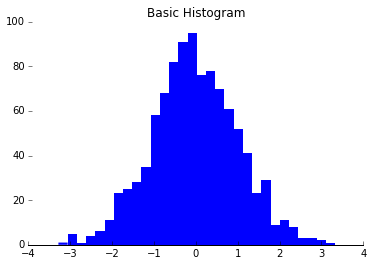
\includegraphics[width=\textwidth]{good_hist_example.png}
\end{subfigure}
\centering
\begin{subfigure}{.45\textwidth}
\centering
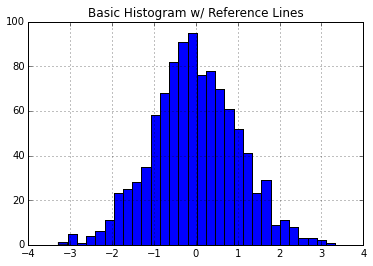
\includegraphics[width=\textwidth]{hist_reference_grid.png}
\end{subfigure}
\caption{Histogram with and without reference lines. It is harder to see the shape of the distribution in the histogram with reference lines.}
\label{fig:histogram}
\end{figure}

A histogram depicts a distribution of numerical data.
The data are sorted into ``bins'' based on what range they lie in.
The height of each vertical bar represents the number of data points in each bin.
A histogram with only a few bins or too many bins will fail to give a clear view of the distribution of the data, therefore it is important to choose the number of bins that gives the best view of the distribution of the data.

Similarly, reference lines are distracting and focus on unnecessary details instead of the shape of the distribution.
If more precise details are desired, exact figures can be presented alongside the histogram in a table.

Use \li{plt.hist()} to create a Matplotlib histogram.


\begin{lstlisting}
from numpy.random import randn
from matplotlib import pyplot as plt

data = randn(75) + randn(75) + randn(75) + randn(75)
plt.hist(data, bins=30)

plt.title("histogram")
plt.show()

\end{lstlisting}

\begin{problem} % Problem: Histograms. TODO: Needs a real data set.
Plot two histograms with data drawn randomly from a normal and exponential distribution.

\begin{lstlisting}
from numpy.random import normal
from numpy.random import exponential
normal_data = normal(size=1000)
exp_data = exponential(size=1000)
\end{lstlisting}

For each distribution, plot a histogram using 30 bins, 15 bins and 5 bins.
Does this change how we interpret the distribution of the data?
\end{problem}

\subsubsection*{Line Plots} % -------------------------------------------------

\begin{figure}[H] % Line plots.
\centering
\begin{subfigure}{.45\textwidth}
\centering
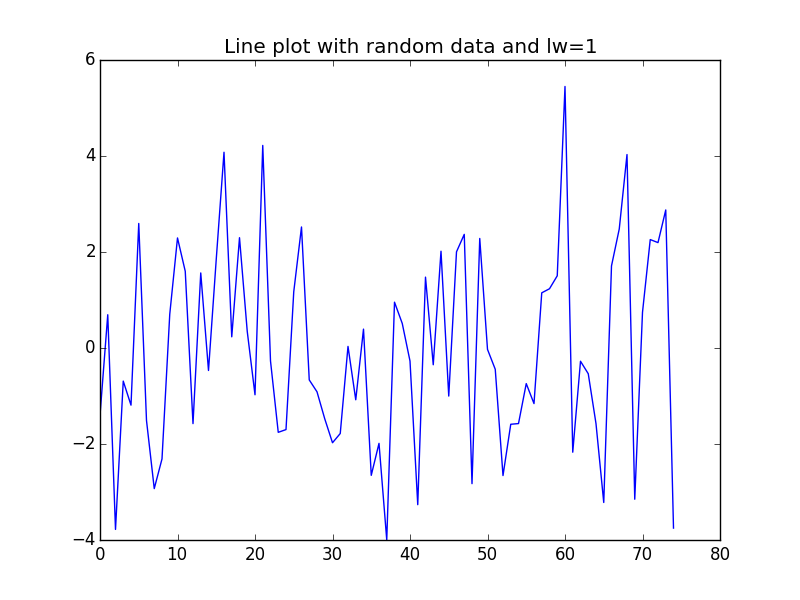
\includegraphics[width=\textwidth]{line_plot_bad_thin.png}
\end{subfigure}
\begin{subfigure}{.45\textwidth}
\centering
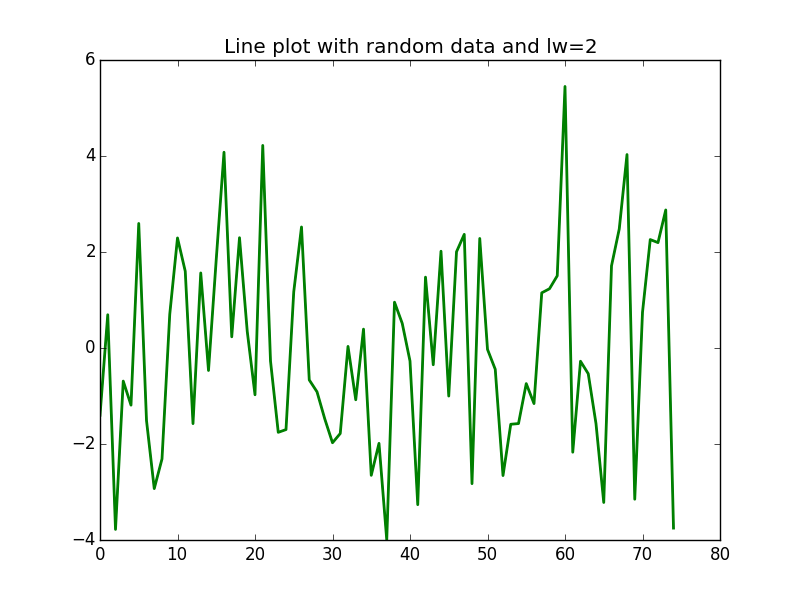
\includegraphics[width=\textwidth]{line_plot_good.png}
\end{subfigure}
\caption{Line Plot.  The left plot is plotted with \li{lw=1} whereas the right plot is plotted with \li{lw=2}.  Notice that the right plot is better because it is easier to see the line.}
\label{fig:lineplot_bad}
\end{figure}

A line plot represents $(x,y)$-pairs as points and connects them with a curve. 
This works well with continuous functions or when there is a natural order in two-dimensional data, for example when the data is a sequence of values over time.
Line plots should \emph{not} be used for data that is one-dimensional or is two-dimensional with no natural
progression (see Figure \ref{fig:lineplotbadX}). % TODO: warning box?

\begin{figure}[H]
\centering
\begin{subfigure}{.5\textwidth}
\centering
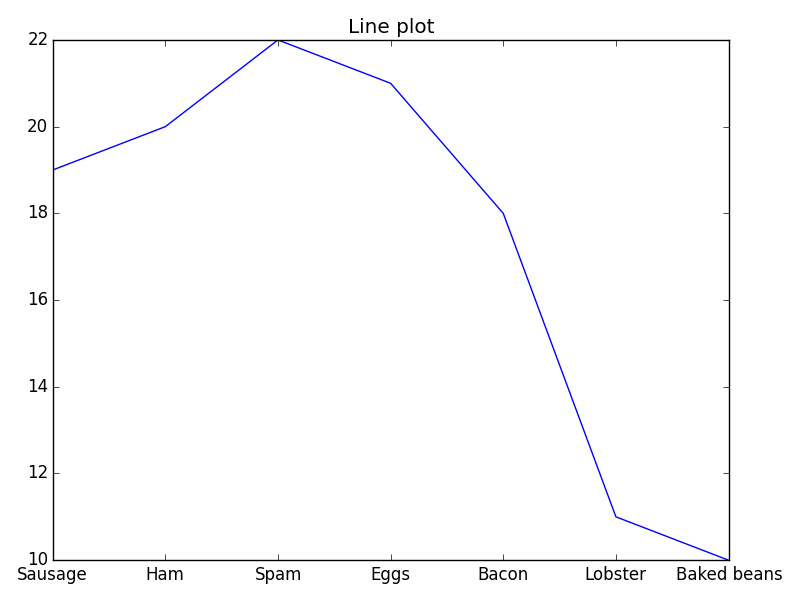
\includegraphics[width=\textwidth]{line_plot_bad_X.png}
\end{subfigure}
\caption{Line plot.  Notice that this graph appears to show that the x-values are ordered.  However, in reality, they are unordered.  This is a bad practice and misrepresents the data.}
\label{fig:lineplotbadX}
\end{figure}

You can create a line plot in Matplotlib with the command \li{plt.plot()}.

\newpage

\subsubsection*{Scatter Plots} % ----------------------------------------------

\begin{figure}[h]
\centering
\begin{subfigure}{.45\textwidth}
\centering
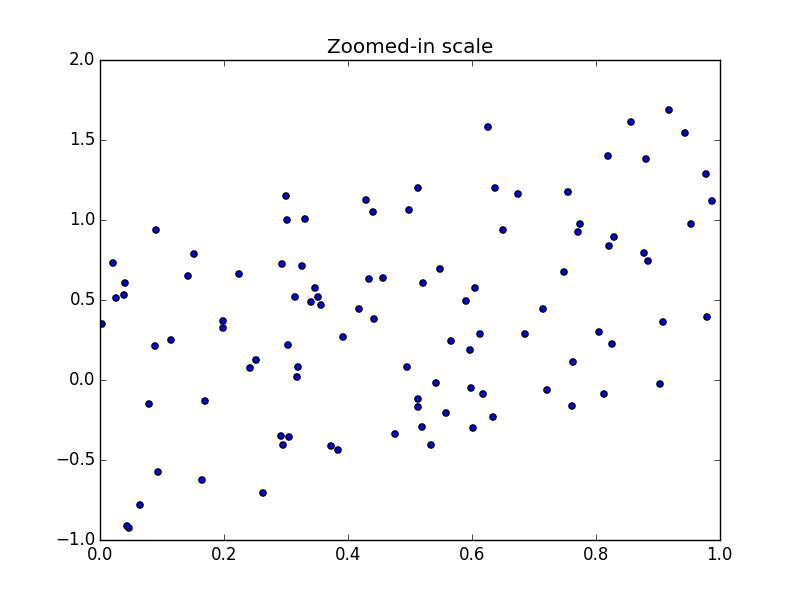
\includegraphics[width=\textwidth]{scale_scatter_zoomed_in.png}
\end{subfigure}
\begin{subfigure}{.45\textwidth}
\centering
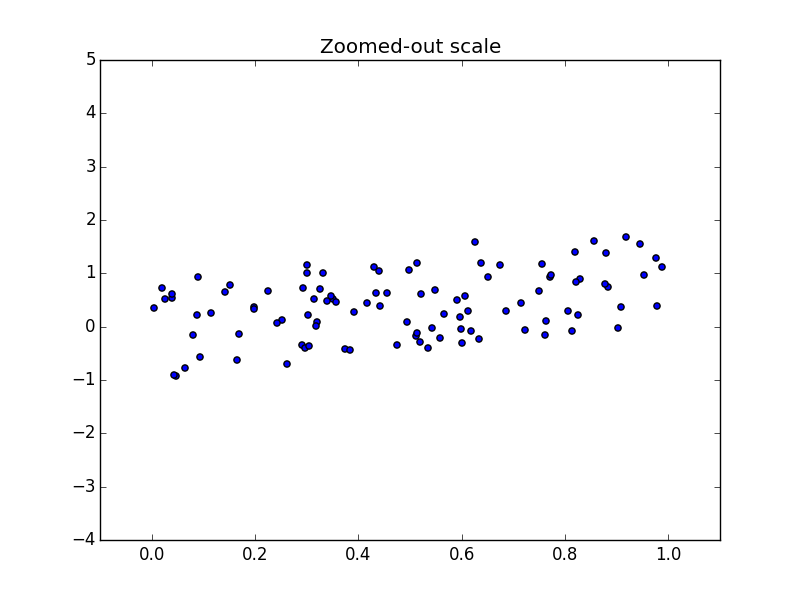
\includegraphics[width=\textwidth]{scale_scatter_zoomed_out.png}
\end{subfigure}
\caption{Scatter Plots.  The data in both plots are the same but there appears to be a weaker
correlation in the first plot compared to the second.}
\label{fig:scatter_correlation}
\end{figure}

Scatter plots graph $(x,y)$ tuples and should be used instead of line plots when the data is two-dimensional but has no natural order.

Figure \ref{fig:scatter_correlation} displays two scatter plots.
The first appears to have a weak correlation and the second appears to have a strong correlation.
However, the same data is being plotted and the only difference is the scale and window size.
Manipulating these can change your interpretation and should be done with careful consideration.

\begin{figure}[h]
\centering
\begin{subfigure}{.45\textwidth}
\centering
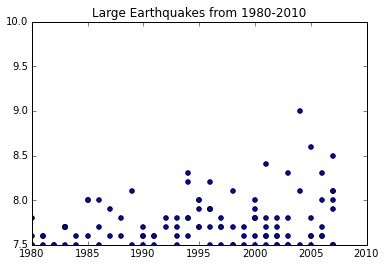
\includegraphics[width=\textwidth]{earthquake_zoomed.png}
\end{subfigure}
\begin{subfigure}{.45\textwidth}
\centering
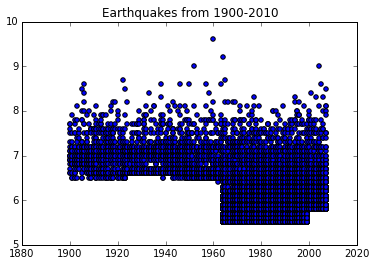
\includegraphics[width=\textwidth]{earthquake_data.png}
\end{subfigure}
\caption{USGS Earthquake data. The scatter plot on the left only plots earthquakes with
magnitude 7.5 or greater from 1980-2010 and appears to have a correlation. 
However, the plot on the right shows all recorded earthquakes from 1900-2010 and shows that the correlation
is not a true correlation.}
\label{fig:scatterquake}
\end{figure}

Scatter plots may reveal insights other than correlation.
Consider Figure \ref{fig:scatterquake} which plots earthquake data from the United States Geological Survey (USGS).
The USGS data began including earthquakes with magnitude 6.5 or greater; this is clearly seen 
in the scatter plot of the entire dataset.
Plots like this may also reveal errors in the dataset that are harder to detect in a table of values.
 
You can create a scatter plot in Matplotlib with the command \li{plt.scatter()}.

\newpage

\subsubsection*{Contour Plots and Heat Maps} % --------------------------------

\begin{figure}[H]
\centering
\begin{subfigure}{.45\textwidth}
\centering
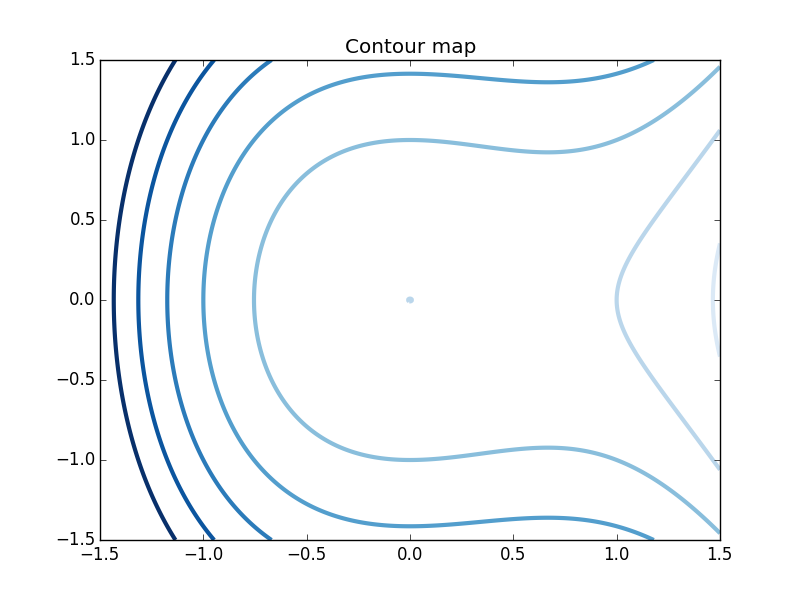
\includegraphics[width=\textwidth]{contour_map.png}
\end{subfigure}
\begin{subfigure}{.45\textwidth}
\centering
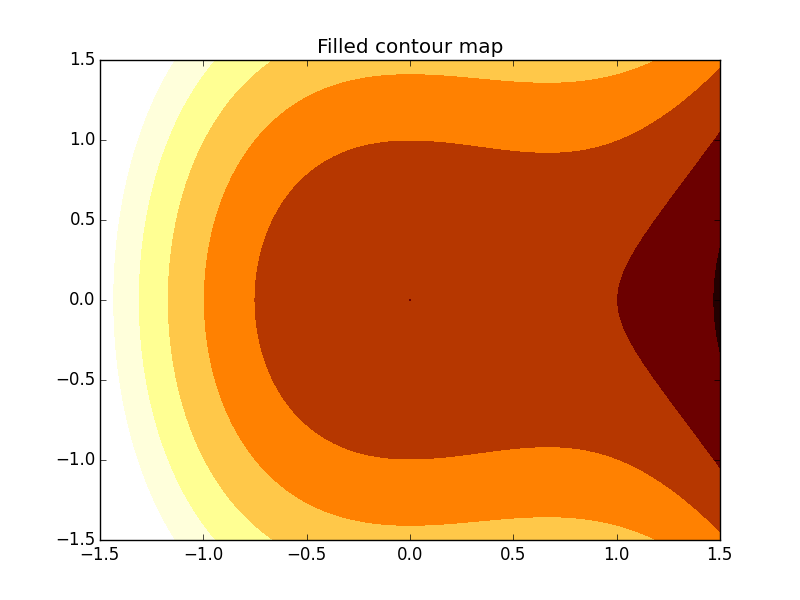
\includegraphics[width=\textwidth]{contour_map_filled.png}
\end{subfigure}
\begin{subfigure}{.45\textwidth}
\centering
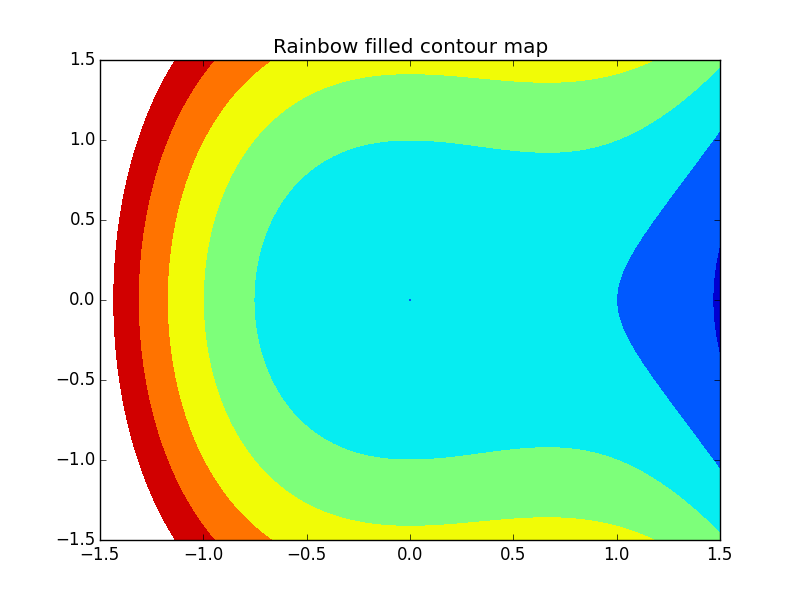
\includegraphics[width=\textwidth]{contour_map_rainbow_filled.png}
\end{subfigure}
\begin{subfigure}{.45\textwidth}
\centering
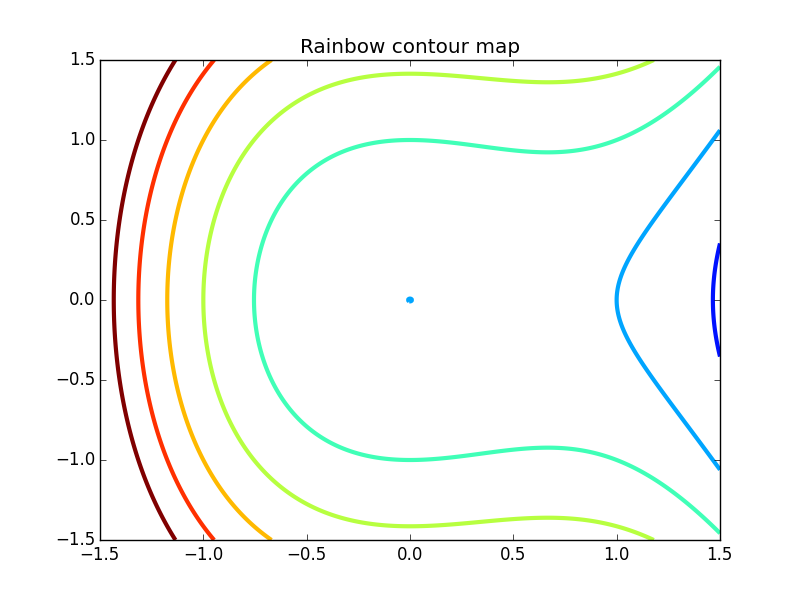
\includegraphics[width=\textwidth]{contour_map_rainbow.png}
\end{subfigure}
\caption{Contour Maps.  A contour map (top left) and a heat map (top right). 
The color choices of the bottom row are less intuitive and make the visualization harder to interpret.}
\label{fig:contour}
\end{figure}


Three-dimensional data can be displayed with a contour plot. 
This draws lines in the plane where the third value is constant---like a topographical map.  
Coloring the space between the contour lines produces a heat map.
Heat maps work best when only one or two colors are used.

\begin{figure}[h]
\centering
\begin{subfigure}{.5\textwidth}
  \centering
  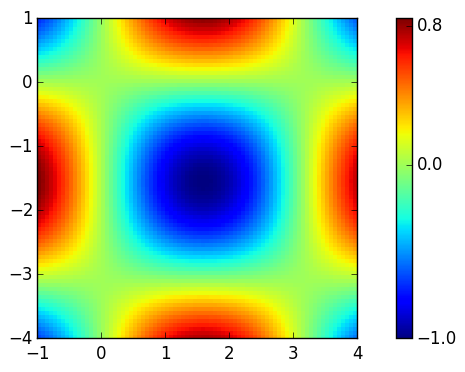
\includegraphics[width=\textwidth]{heatmap_color.png}
\end{subfigure}%
\begin{subfigure}{.5\textwidth}
  \centering
  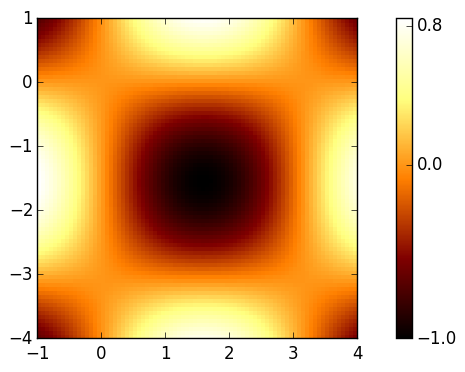
\includegraphics[width=\textwidth]{heatmap_hot.png}
\end{subfigure}
%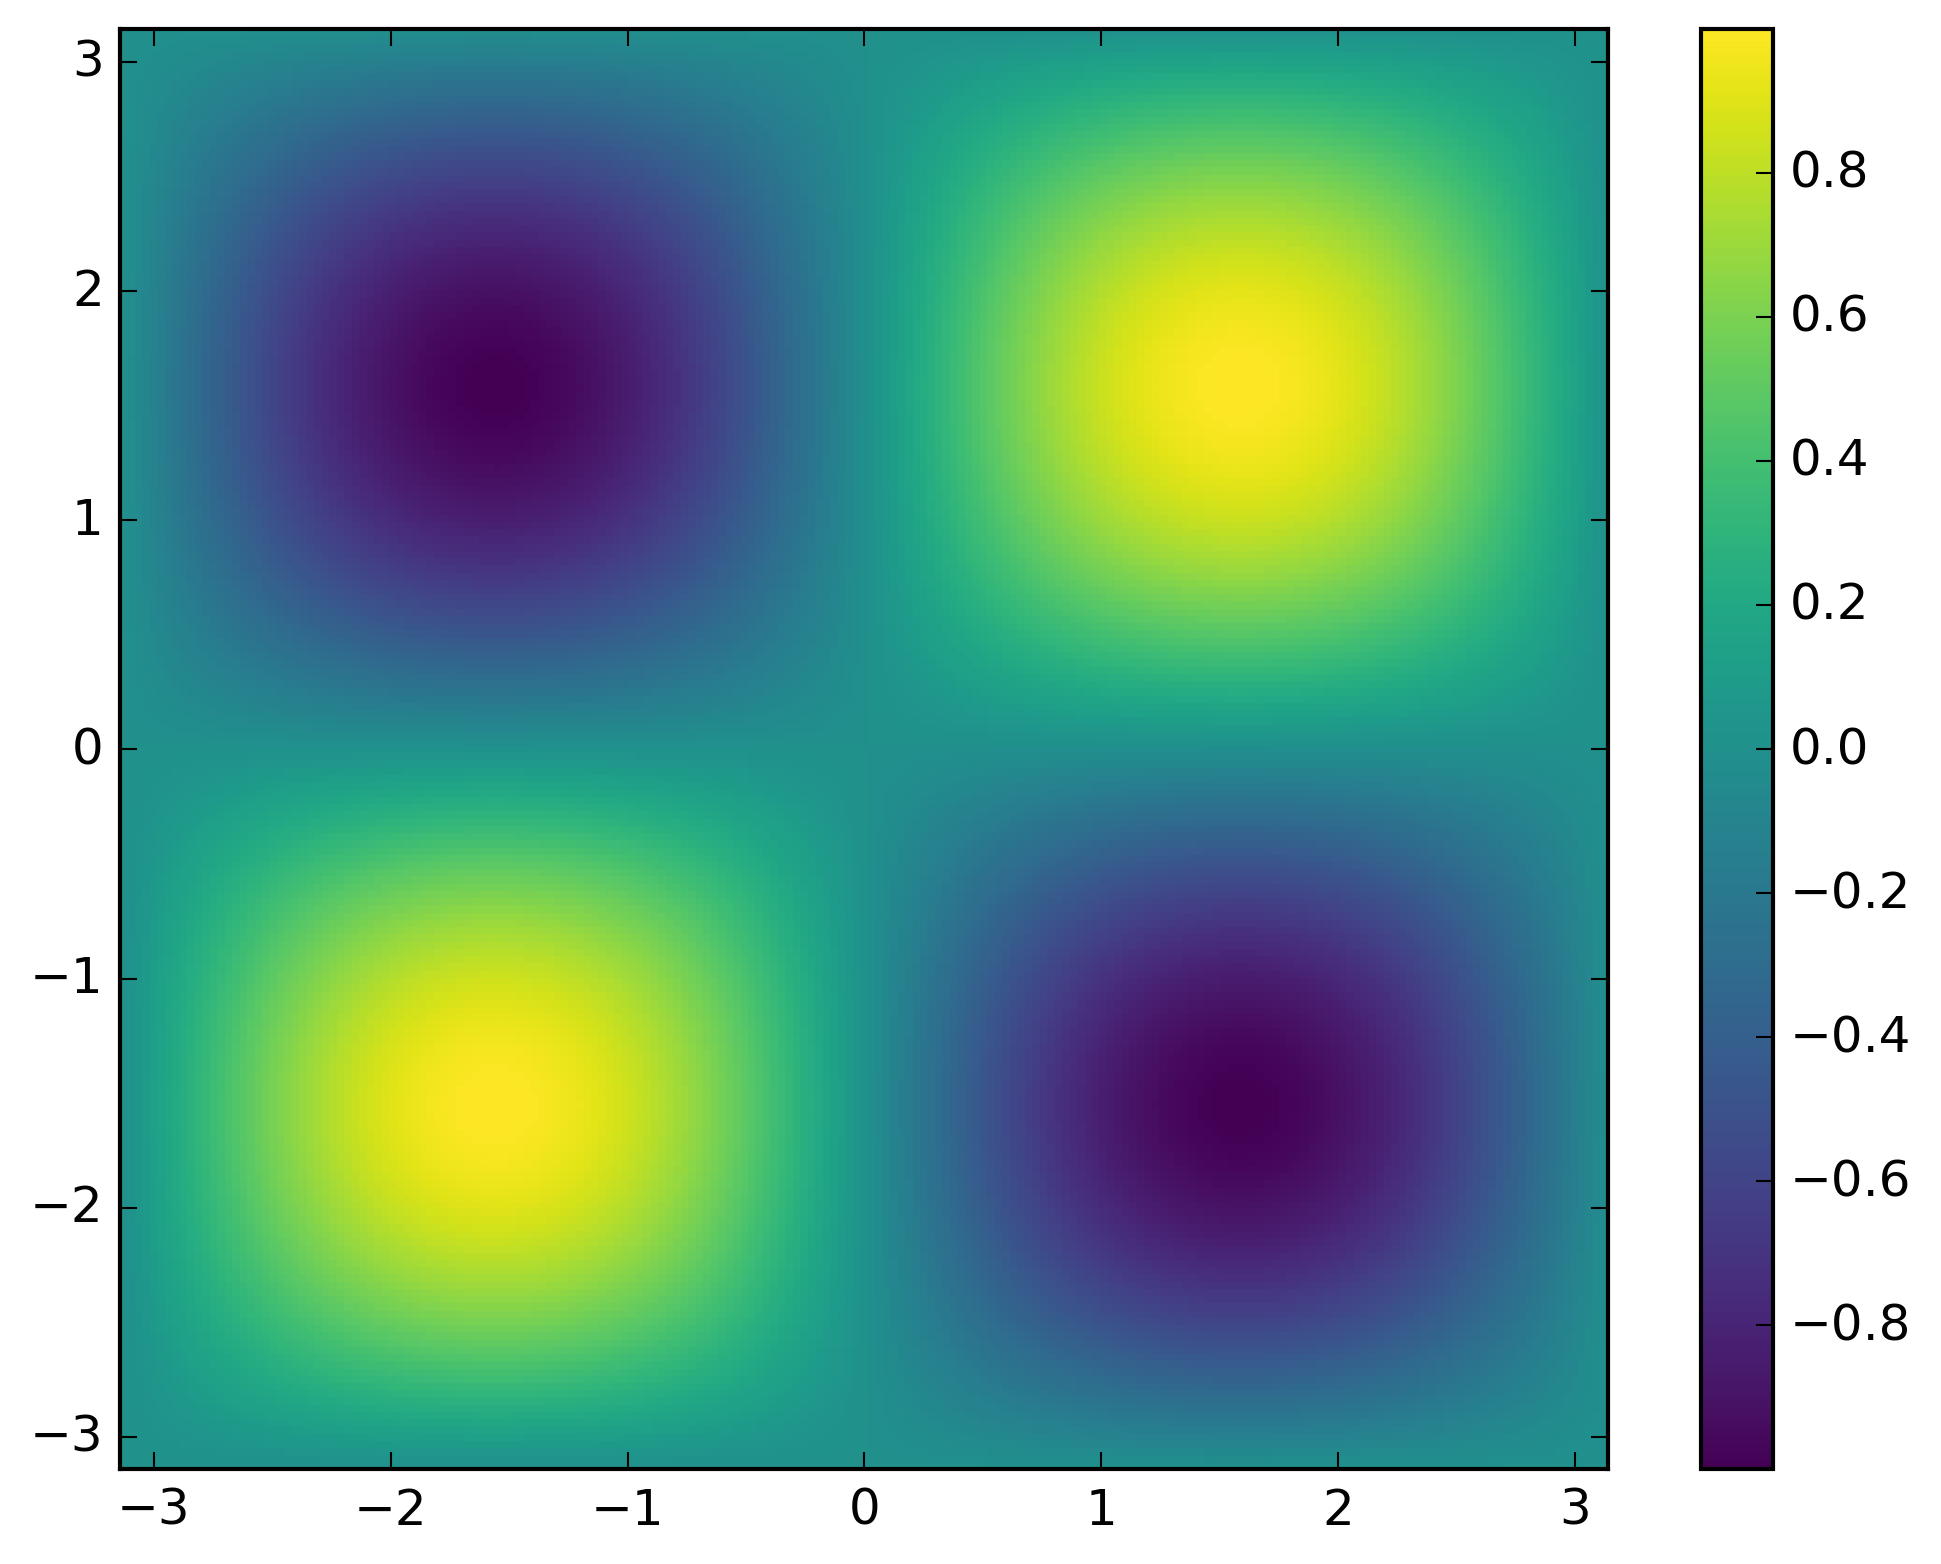
\includegraphics[width=\textwidth]{heatmap.png}
\caption{Both of these pseudocolor plots depict the function
	$z = \sin(x)\sin(y)$ on the domain $[-1,4] \times [-4,1]$. 
The plot on the left uses a rainbow gradient, which has no meaningful relationship to the data. 
The plot on the right uses the colormap \li{afmhot}.  The lighter and darker colors are a more intuitive
representation of higher and lower values.}

\label{fig:heatmap}
\end{figure}

% TODO: In the next release of Matplotlib (version 2.0) viridis is the default.
% TODO: Reword (awkward).
A good default colormap is Matplotlib's \li{viridis}.
Other colormaps that are appropriate for the data can be selected using the argument \li{cmap='NAME\_OF\_COLORMAP'}, where \li{NAME\_OF\_COLORMAP} is one of Matplotlib's sequential or diverging colormaps.
Two sequential colormaps are \li{afmhot} and \li{cool}. Two diverging colormaps are \li{seismic} and \li{bwr}. 
These colormaps along with their color scheme can be found on
\url{http://matplotlib.org/examples/color/colormaps_reference.html}.
Although three-dimensional data can be plotted as a surface in 3-space, it is often difficult to find a view where none of the important features of the data are obscured.
A heatmap avoids this problem and is easier to understand.

You can create a contour plot in Matplotlib with \li{plt.contour()}.

You can also create a pseudocolor plot in Matplotlib with the \li{plt.pcolormesh()} command.

% # This code corresponds to the figure on the top right of the contour maps.
\begin{lstlisting}
import numpy as np
from matplotlib import pyplot as plt

n=400
xran = np.linspace(-1.5,1.5,n)
yran = np.linspace(-1.5,1.5,n)
X, Y = np.meshgrid(xran,yran)
F = Y**2 - X**3 + X**2
plt.contourf(X, Y, F, [-2,-1,0.0001,1,2,3,4,5] ,cmap=plt.get_cmap('afmhot'))
\end{lstlisting}

\begin{problem} % Contour map problem. TODO: don't specify number of intervals?
Using 400 intervals, plot a filled contour map of the function \[f(x,y) = \sin(x) + \sin(y)\] over the domain $[0,12\pi]\times[0,12\pi]$. 

Be sure to use an appropriate color map. 
\end{problem}

\section*{Communicating Insights with Visualizations} % =======================

As in any form of communication, integrity is important in data visualization.
Every visualization should be presented alongside all relevant information including who created it, where the data was obtained, how it was collected, whether it was cleaned or transformed, and whether there are conflicts of
interest or possible biases present.
Where appropriate, use words to carefully explain the insights represented
in the visualization.
These practices will help the reader correctly interpret the visualization.

\subsection*{Things to Avoid} % -----------------------------------------------

Some popular visualizations (pie charts, radar graphs, stacked bar charts and others) interfere with our ability to interpret the information they display.
For example, it is more difficult to detect differences in a pie chart than on a bar chart with the same data.
This is because differences in area are more difficult to detect than differences in length. 
As a result, charts that depend on detecting variation in area will be less effective.
Instead, choose visualizations that compare the data to the a simple standard that is easy to understand and interpret.
Figures \ref{fig:pievsbar} and \ref{fig:stacked} are examples of poorly chosen visualizations.

\begin{figure} % Bad graphs.
\centering
\begin{subfigure}{.45\textwidth}
\centering
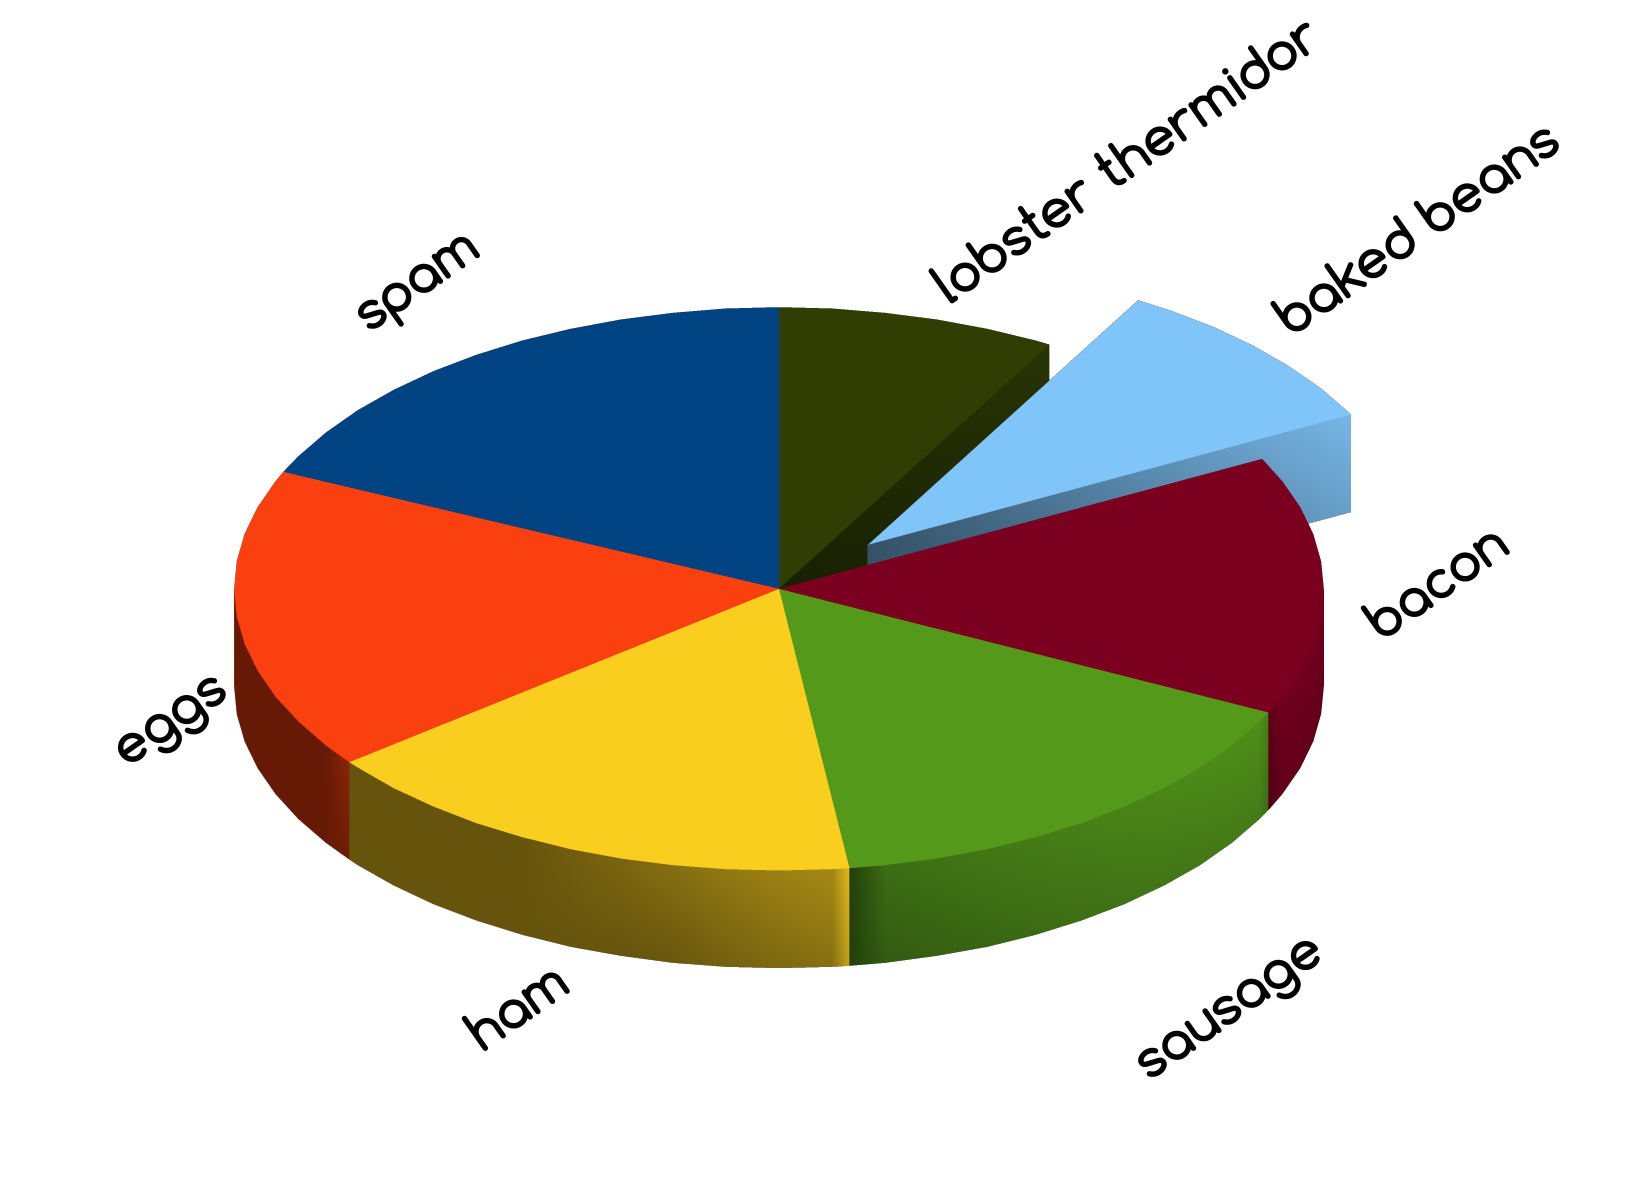
\includegraphics[width=\textwidth]{bad_pie_chart.png}
\end{subfigure}
\begin{subfigure}{.45\textwidth}
\centering
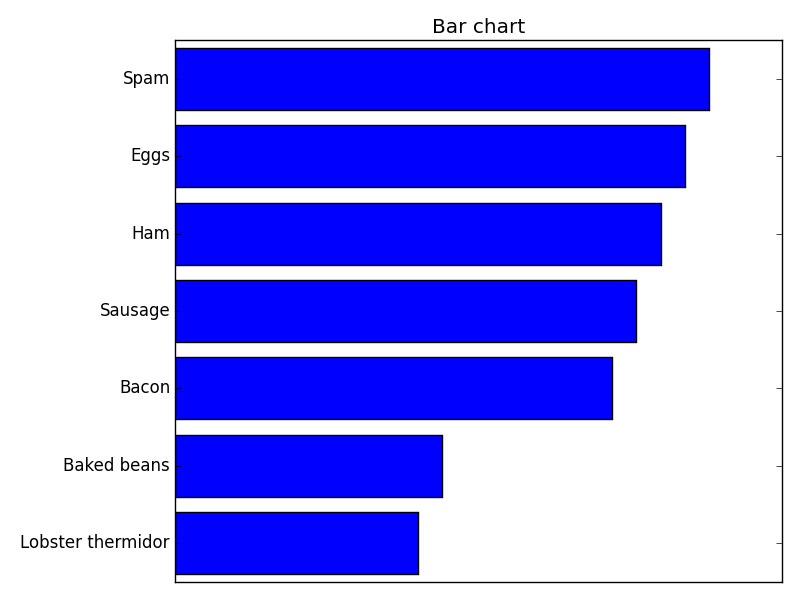
\includegraphics[width=\textwidth]{bar_chart_horizontal_sorted.png}
\end{subfigure}
\caption{A pie chart on the left that has been improved by a transformation into a bar chart on the right.}
\label{fig:pievsbar}
\end{figure}

\subsection*{Keep It Simple} % ------------------------------------------------

It may be tempting to stylize your visualization by adding icons and pictures or by making certain features
look 3D.  This is called chartjunk, a term coined by Edward Tufte. Chartjunk is anything in a plot that fails to add to or
misrepresents the data.  Avoid making visualizations that are overly fancy or cluttered with chartjunk. This
includes 3D effects (as in \ref{fig:pievsbar}), bad font choices, and unnecessary icons and pictures.
Visualizations are at their best when they are as simple as possible and allow the reader to easily
interpret the information being presented.

Reference lines can distract from the visualization (see Figure \ref{fig:histogram}).
For example, we can remove axis lines, tick marks, and bar lines
with the following code:

\begin{lstlisting}
# Get current axis instance
axis = plt.gca()

# Hide top and right spines
axis.spines['right'].set_visible(False)
axis.spines['top'].set_visible(False)

# Only show bottom and left tick marks
axis.yaxis.set_ticks_position('left')
axis.xaxis.set_ticks_position('bottom')
\end{lstlisting}

\begin{problem} % Problem: convert a pie chart to a horizontal bar chart.
Regraph the pie chart in Figure \ref{fig:pievsbar} as a horizontal bar chart using the follwing data.
Spam: 21, Eggs: 20, Ham: 22, Sausage: 21, Bacon: 20, Baked Beans: 11, Lobster Thermidor: 10
\end{problem}

% TODO: WHY IS THIS PROBLEM WAY DOWN HERE??? Shouldn't this be part of the histogram section?
\begin{problem} % Problem: histogram of earthquake magnitudes.
Plot a histogram of earthquake magnitudes using the data in the file \li{earthquake.txt}. 
Remove reference lines, tick marks and bar lines.
Use the numpy function \li{np.loadtxt()} to read in the data.
Is the data distributed normally or exponentially?
\end{problem}

\begin{figure} % Stacked v unstacked bar charts
\centering
\begin{subfigure}{.45\textwidth}
\centering
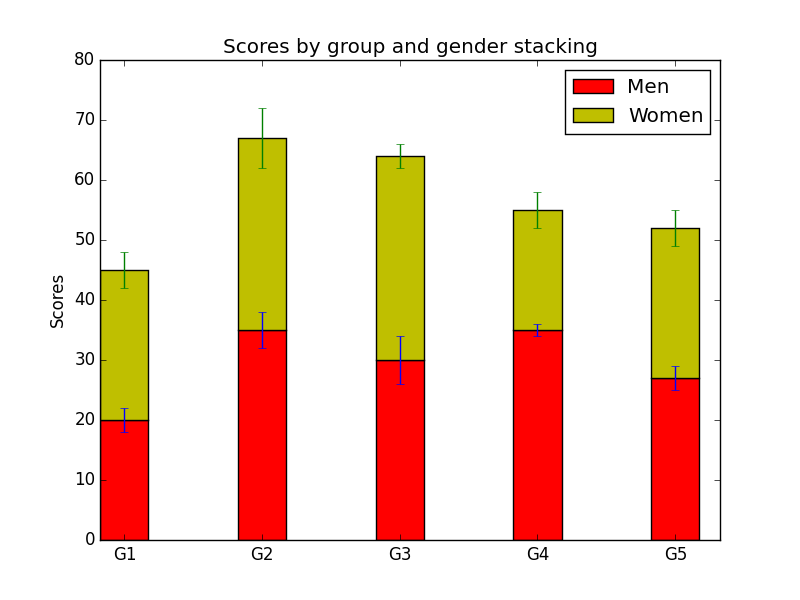
\includegraphics[width=\textwidth]{stackedbar.png}
\end{subfigure}
\begin{subfigure}{.45\textwidth}
\centering
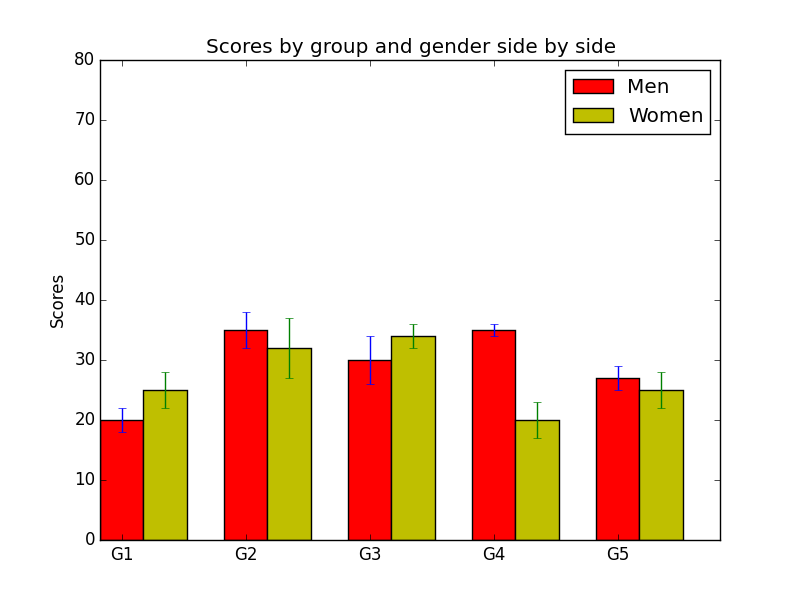
\includegraphics[width=\textwidth]{unstackedbar.png}
\end{subfigure}
\caption{Stacked Bar Chart. The relative values are harder to compare when stacked (left) instead of adjacent (right).}
\label{fig:stacked}
\end{figure}

\subsection*{Small Multiples} % -----------------------------------------------

When we have too much information to display cleanly in one chart, we can split the visualization into many smaller visualizations and place them near each other so they can be easily compared.
This method is called \emph{small multiples} and was made famous by Edward Tufte.

As an example, consider the first six Chebyshev polynomials.
Plotting them all on the same graph makes the visualization cluttered.
Instead, each polynomial can be given its own graph and laid out in a way that makes them easy to compare, (see Figure \ref{fig:PoT}).

% add more reference material??

\begin{figure} % Chebyshev polynomials
\centering
\begin{subfigure}{.45\textwidth}
  \centering
  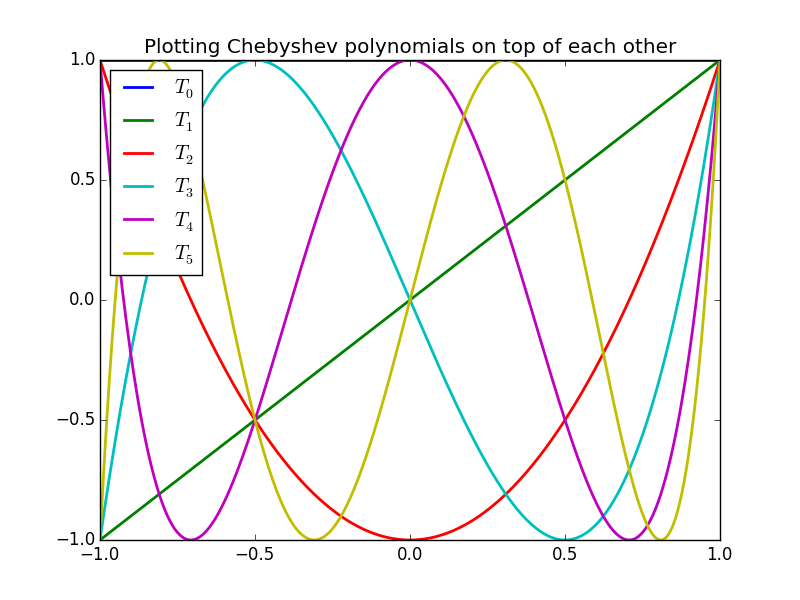
\includegraphics[width=\textwidth]{PoT.png}
\end{subfigure}
\begin{subfigure}{.45\textwidth}
\centering
  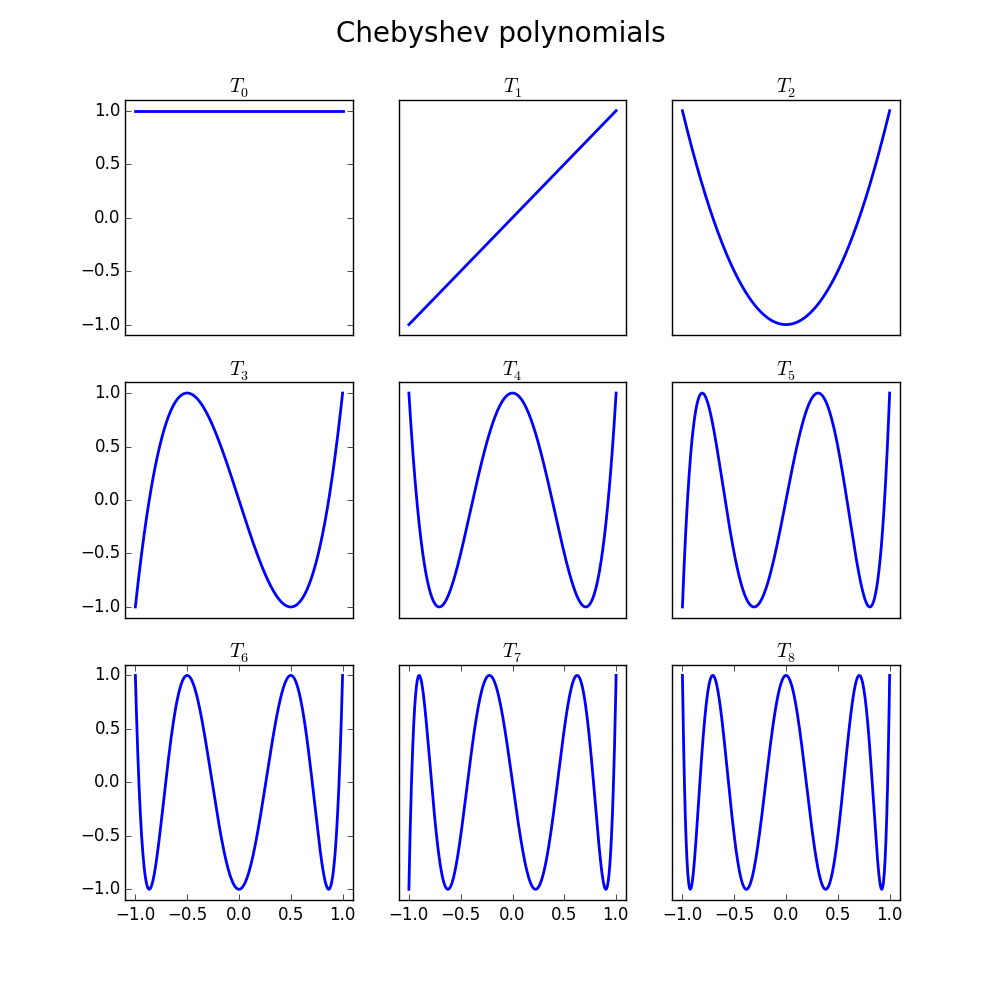
\includegraphics[width=\textwidth]{PoT_separate.png}
\end{subfigure}
\caption{Chebyshev polynomials graphed together on the left and in small multiples on the right.
The small multiples are much easier to interpret.}
\label{fig:PoT}
\end{figure}

To make small multiples, use the Matplotlib command \li{ax = plt.subplot()} which sets up multiple plots one at a time.
% Some example code is provided below.

\begin{lstlisting}
import numpy as np
from matplotlib import pyplot as plt
from numpy.polynomial import Chebyshev as T

def Chebyshev_subplots():
    fig = plt.figure(dpi=100)
    fig.set_size_inches(10,10)
    fig.suptitle('Chebyshev Polynomials', fontsize=20)

    x = np.linspace(-1,1,500)

    for i in range(9):
        ax = plt.subplot(3,3,i+1)
        ax.plot(x, T.basis(i)(x), lw=2, label="$T_%d$"%i)
        plt.xlim(-1.1,1.1)
        plt.ylim(-1.1,1.1)
        ax.set_title('$T_%d$'%i)
        if i%3:
            # remove the inner y-ticks and labels.
            ax.set_yticklabels([])
            ax.yaxis.set_ticks_position('none')
        if i<6:
            # remove the inner x-ticks and labels.
            ax.xaxis.set_ticks_position('none')
            ax.set_xticklabels([]) 

    plt.show()
\end{lstlisting}

\begin{problem} % Problem: plot the Bernstein polynomials.
The $n+1$ Bernstein basis polynomials of degree $n$ are defined as 

$$b_{v,n} = {{n} \choose {v}} x^v (1-x)^{n-v}, v = 0, 1,..., n.$$

Plot the Bernstein basis polynomials for $v,n$ in [0,3] as small multiples and compare that to the cluttered version of plotting them on top of each other.
\end{problem}

% \begin{comment}

\subsection*{Additional Material} % ===========================================

There are many software packages that facilitate the visual exploration of data. 
One Python library is Glue (see \cite{glue}).

Some packages for making nicer looking plots include \li{Seaborn} and \li{prettyplotlib}.  TODO get refs

For more about visualization of data, we highly recommend the following books:

TODO get full refs for the follwoing

\begin{itemize}
\item \emph{How to lie with statistics}
\item \emph{Envisioning Information} by Edward Tufte
\item \emph{The visual display of quantitative information} by Edward Tufte (2nd edition)
\item \emph{Beautiful Evidence} by Edward Tufte
\item \emph{Now you see it} by Stephen Few
\end{itemize}

% \end{comment}

\printbibliography
